\documentclass[english, xcolor={table,usenames}]{beamer}
\usepackage{graphicx}
\usepackage[english]{babel}
\usepackage[utf8]{inputenx}
\usepackage[T1]{fontenc}      % Font encoding
\usepackage{palatino}          % lmodern font, correctly copyable characters in pdf
\usepackage{hyperref}         % Hyperlinks
\usepackage{amsmath}          % Math
\usepackage{amssymb}          % Math symbols
\usepackage{mathtools}        % Math tools
\usepackage{siunitx}          % SI units
\usepackage{microtype}        % Microtypography
\usepackage{bookmark}
\usepackage{subfigure}
\usepackage{tikz}
\usepackage{chngcntr}
\usepackage{ragged2e}
\counterwithin{subfigure}{figure}
\usepackage{caption}
\usepackage{listings}
\usepackage[binary-units]{siunitx}
\usepackage{tabularx}
\usepackage{booktabs}         % Tables
\usepackage{float}
\usepackage{listings}
\usepackage{bera}
\usepackage{cleveref}

%%%% COMPILE WITH LATEXMK %%%%

\usetheme[
  bullet=circle,                  % Use circles instead of squares for bullets
  titleline=false,                % Show a line below the frame
  alternativetitlepage=true,      % Use the fancy title
  titlepagelogo=logo-sapienza,    % Logo for the first slide
  watermark=watermark-diag,       % Watermark used in every slide
  watermarkheight=20px,           % Desired height of the watermark
  watermarkheightmult=6,          % Watermark image is actually x times bigger
  displayauthoronfooter=true,     % Display author name in the footer
]{Roma}
\watermarkoff%
\author{\textbf{Dario Loi} --- \textbf{1940849}}

\title{Multi-Lingual Natural Language Processing}
\subtitle{Homeworks Report}
\institute{M.Sc. in AI \& Robotics, \\ Sapienza, University of Rome.}
\date{A. Y. 2023--2024}

% Cover future items, do not cover past items

\setbeamercovered{transparent=20}

\colorlet{punct}{red!60!black}
\definecolor{background}{HTML}{EEEEEE}
\definecolor{delim}{RGB}{20,105,176}
\colorlet{numb}{magenta!60!black}
\lstdefinelanguage{json}{
    basicstyle=\tiny\normalfont\ttfamily,
    numbers=left,
    numberstyle=\tiny,
    stepnumber=1,
    numbersep=8pt,
    showstringspaces=true,
    breaklines=true,
    frame=lines,
    backgroundcolor=\color{background},
    literate=
     *{0}{{{\color{numb}0}}}{1}
      {1}{{{\color{numb}1}}}{1}
      {2}{{{\color{numb}2}}}{1}
      {3}{{{\color{numb}3}}}{1}
      {4}{{{\color{numb}4}}}{1}
      {5}{{{\color{numb}5}}}{1}
      {6}{{{\color{numb}6}}}{1}
      {7}{{{\color{numb}7}}}{1}
      {8}{{{\color{numb}8}}}{1}
      {9}{{{\color{numb}9}}}{1}
      {:}{{{\color{punct}{:}}}}{1}
      {,}{{{\color{punct}{,}}}}{1}
      {\{}{{{\color{delim}{\{}}}}{1}
      {\}}{{{\color{delim}{\}}}}}{1}
      {[}{{{\color{delim}{[}}}}{1}
      {]}{{{\color{delim}{]}}}}{1},
}


\begin{document}

\maketitle

\section{Homework 1-A}

\subsection{Introduction}
\begin{frame}{Tasks}
  For the first homework, we were assigned \alert{two} datasets:

  \begin{enumerate}
    \item WiC-ITA: Detect whether two italian words in two \alert{different} sentences are used with the \alert{same} meaning.
    \item ITAmoji: Predict which emoji was used in a given italian tweet.
  \end{enumerate}

  For each, we need to transform the samples into a format that is suitable for training an LLM, we also need to
  write the prompts that the model will use to make predictions. Additionally, we need to generate \alert{distractors} for the ITAmoji dataset.
\end{frame}


\begin{frame}[fragile]{WiC-ITA}
  The first dataset's original samples' schema is shown in \cref{lst:wic}.
  \begin{figure}[H]
    \centering

    \begin{lstlisting}[language=json, escapeinside = {(*@}{@*)}, caption={Sample 23 from WiC-ITA \texttt{train.jsonl}.}, label={lst:wic}]
  {
    "id": "lira.noun.15",
    "lemma": "lira",
    "sentence1": "In caso di inosservanza degli obblighi stabiliti dal comma 1 , si applica la sanzione amministrativa pecuniaria da lire dieci milioni a lire cento milioni .",
    "sentence2": "Per le finalit(*@\`{a}@*) di cui all' Art. 1 , comma 2 , della legge regionale 26 aprile 1995 , n. 31 recante \" Norme in materia di musei degli Enti locali e di interesse locale \" (*@\`{e}@*) autorizzata per l' esercizio finanziario 2000 la spesa di lire 200.000.000 .",
    "start1": 115,
    "end1": 119,
    "start2": 230,
    "end2": 234,
    "label": 1
  }
  \end{lstlisting}
  \end{figure}

\end{frame}

\begin{frame}[fragile]{Desired Format}

  The desired schema is shown in \cref{lst:wic_desired}.


  \begin{figure}[H]
    \centering
    \begin{lstlisting}[language=json, escapeinside = {(*@}{@*)}, caption={Same sample with required changes.}, label={lst:wic_desired}]
  {
    "id": "lira.noun.15",
    "lemma": "lira",
    "sentence1": "In caso di inosservanza degli obblighi stabiliti dal comma 1 , si applica la sanzione amministrativa pecuniaria da lire dieci milioni a lire cento milioni .",
      "sentence2": "Per le finalit(*@\`{a}@*) di cui all' Art. 1 , comma 2 , della legge regionale 26 aprile 1995 , n. 31 recante \" Norme in materia di musei degli Enti locali e di interesse locale \" (*@\`{e}@*) autorizzata per l' esercizio finanziario 2000 la spesa di lire 200.000.000 .",
    "start1": 115,
    "end1": 119,
    "start2": 230,
    "end2": 234,
    "choices": [
      "DIVERSO",
      "UGUALE"
    ],
    "label": 1
  }
\end{lstlisting}
  \end{figure}
\end{frame}

\begin{frame}[fragile]{ITAmoji}
  The second task's JSON schema is shown in \cref{lst:itamoji}.
  \begin{figure}[H]
    \centering
    \begin{lstlisting}[language=json, escapeinside = {(*@}{@*)}, caption={Sample 27 from \texttt{ITAmoji\_2018\_TRAINdataset\_v1.ANON.list}.}, label={lst:itamoji}]
  {
    "uid": "447352763",
    "text_no_emoji": "... il rumore del mare \ufe0f #28Settembre <URL>",
    "created_at": "Thu Sep 28 15:32:06 +0000 2017",
    "label": "red_heart",
    "tid": "913426094002458626"
  }
  \end{lstlisting}
  \end{figure}

  For this task, we also had to add \alert{distractors}, that is, plausible alternatives to the correct label.

\end{frame}


\begin{frame}[fragile]{Desired Format... Again}
  The desired output, with generated distractors, is shown in \cref{lst:itamoji_desired}.

  \begin{figure}[H]
    \centering
    \begin{lstlisting}[language=json, escapeinside = {(*@}{@*)}, caption={Sample 27 with generated distractors.}, label={lst:itamoji_desired}]
  {
    "id": "ITA-emoji-train-00000027",
    "sentence": "... il rumore del mare \ufe0f #28Settembre <URL>",
    "choices": [
        "red_heart",
        "two_hearts",
        "rose",
        "kiss_mark"
    ],
    "label": 0
  }
  \end{lstlisting}
  \end{figure}
\end{frame}

\begin{frame}{Distractor Clusters}
  To generate distractors, we used a hand-crafted list of \alert{semantic clusters}, which we define as
  a set of emoji that are semantically related. For example, the cluster \texttt{love} contains the
  emojis \texttt{red\_heart}, \texttt{two\_hearts}, \texttt{blue\_heart}, \texttt{rose}, and \texttt{kiss\_mark}.

\end{frame}

\begin{frame}{Distractor Sampling}
  To obtain a set of distractors from an ITAmoji sample, we follow this process:

  \begin{itemize}
    \item<1-> Randomly sample a cluster from the list of clusters that contain the correct emoji.
    \item<2-> Randomly sample three other emojis from the same cluster.
    \item<3-> Return the new sample with the correct label and the three distractors.
  \end{itemize}
\end{frame}


\begin{frame}[fragile]
  \frametitle{Prompts}
  For both tasks, we adopted an \emph{Chain-of-Thought} approach, where we show a couple of
  correct examples to the model before asking it to make predictions.

  In the next slides we will show examples of this approach applied to both tasks.
\end{frame}


\begin{frame}[fragile]
  \frametitle{WiC-ITA Prompts}

  Here is an example of a prompt for the WiC-ITA dataset:

  \tiny\begin{verbatim}
  Il tuo compito e' effettuare delle classificazioni su un sample di un dataset Word in Context.
  L'input consiste in due frasi e una parola, 
  l'output e' una classificazione binaria che indica se il significato della parola 
  e' diverso (0) o lo stesso (1) nelle due frasi.
  Adesso elenchero una serie di esempi, per l'ultimo esempio dovrai completare la classificazione.
  Fai attenzione a rispondere solo con 0 se la scelta e' "DIVERSO" 
  o 1 se la scelta e' "UGUALE", non scrivere altro. 
  
  Parola: RE
  Frase 1: "Carlo magno fu incoronato re dei romani ad aquisgrana"
  Frase 2: "La scala maggiore di re ha due alterazioni, fa e do"
  Risposta corretta: 0
  
  Parola: ARCO
  Frase 1: "L'arco di trionfo e' uno dei monumenti più famosi di parigi"
  Frase 2: "Grazie all'invenzione dell'arco di volta, 
  i romani erano capaci di costruire monumenti impressionanti"
  Risposta corretta: 0

  Parola: {{lemma}}
  Frase 1: {{sentence1}}
  Frase 2: {{sentence2}}
  Risposta corretta:
\end{verbatim}
\end{frame}


\begin{frame}[fragile]
  \frametitle{ITAmoji Prompts}

  Here is an example of a prompt for the ITAmoji dataset:

  \tiny\begin{verbatim}
  Il tuo compito e' quello di identificare l'emoji corretta 
  associata a un tweet prodotto da un utente italiano, 
  ti verranno fornite tre opzioni tra cui scegliere, 
  una delle quali e' corretta. Le opzioni sono simili tra di loro, 
  quindi presta attenzione ai dettagli.

  Ecco alcuni esempi, completa l'ultimo rispondendo solo con l'emoji corretta.

  Tweet: <MENTION_1> Avete visto cosa ha fatto il governo? <MENTION_2> #governo #italia
  Scelte: ["thinking_face", "face_screaming_in_fear", "face_with_tears_of_joy"]
  Risposta: thinking_face

  Tweet: Ho dimenticato le chiavi in Macchina!!! Maledizione!!
  Scelte: ["face_with_tears_of_joy", "face_screaming_in_fear", "loudly_crying_face"]
  Risposta: face_screaming_in_fear

  Tweet: {{sentence}}
  Scelte: {{choices}}
  Risposta:
\end{verbatim}

\end{frame}

\section{Homework 1-B}

\begin{frame}
  \frametitle{Homework 1-B}

  The second homework required the training of some classifier models on the HaSpeeDe dataset,
  in order to detect whether a given sentence is \alert{hateful} or \alert{non-hateful}.

  We were provided \alert{two} datasets, one on news articles and one on tweets, both in
  the Italian language.
\end{frame}

\begin{frame}
  \frametitle{The Models}

  The models we trained were:

  \begin{enumerate}
    \item<1-> A naïve classifier that always predicts the majority class.
    \item<2-> A Logistic Regression model that operates on Word2Vec embeddings.
    \item<3-> An LSTM model that automatically learns embeddings.
  \end{enumerate}

\end{frame}

\begin{frame}
  \frametitle{Naïve Classifier}

  The naïve classifier always predicted the \alert{non-hateful} label, and achieved
  an accuracy of $0.638$ on the news dataset and $0.508$ on the tweets dataset.

  We naturally achieved \alert{perfect} precision, with a recall equal to that
  of the accuracy.
\end{frame}

\begin{frame}
  \frametitle{Word2Vec Regression}

  For the embeddings, we used the \texttt{gensim} library to train a Word2Vec model
  on the training data, with an embedding size of $300$. We do \alert{not} use pre-trained embeddings since the semantic meaning of
  some of the words differ from those of general language (we notice a general anti-establishment
  sentiment in the hateful tweets that we want to capture).

  The Word2Vec embeddings of the sentence's tokens are averaged to obtain a single embedding
  that is then projected by a logistic regression model.
\end{frame}

\begin{frame}
  \frametitle{LSTM Model}

  Our LSTM model employs an embedding layer to automatically learn the embeddings of the words. We used a bidirectional LSTM with an embedding size of $300$ and a hidden size of $128$,

  The model was trained for $5$ epochs with a batch size of $32$, embedding size was set to $300$ (same as Word2Vec), and the hidden size was set to $128$.

\end{frame}

\begin{frame}[fragile]
  \frametitle{Results (News)}

  \begin{figure}[h]
    \centering
    \caption{Results on the news test set}
    \begin{tabular}{|c|c|c|c|c|}
      \hline
      Model               & Accuracy & Precision & Recall & F1    \\
      \hline
      \hline
      Logistic regression & 0.666    & 0.776     & 0.824  & 0.800 \\
      LSTM                & 0.714    & 0.869     & 0.800  & 0.833 \\
      Baseline            & 0.638    & 1.000     & 0.638  & 0.779 \\
      \hline
    \end{tabular}
  \end{figure}

\end{frame}

\begin{frame}
  \frametitle{Results (Tweets)}

  \begin{figure}[h]
    \centering
    \caption{Results on the tweets test set}
    \begin{tabular}{|c|c|c|c|c|}
      \hline
      Model               & Accuracy & Precision & Recall & F1    \\
      \hline
      \hline
      Logistic regression & 0.605    & 0.650     & 0.898  & 0.754 \\
      LSTM                & 0.702    & 0.772     & 0.885  & 0.825 \\
      Baseline            & 0.508    & 1.000     & 0.508  & 0.673 \\
      \hline
    \end{tabular}
  \end{figure}
\end{frame}

\section{Homework 2}

\begin{frame}
  \frametitle{Homework 2}

  The third homework focused on the \alert{Neural Logical Inference} (NLI) task, performed
  on the FEVER dataset. The task consists of determining whether a given hypothesis is
  \alert{supported}, \alert{refuted}, or simply \alert{indeterminate} given a premise that we assume to be true.
\end{frame}

\begin{frame}
  \frametitle{Data Augmentation}

  A key part of the homework was the generation of \alert{adversarial} samples, these samples
  should have a more complex sentence structure than the original sample, in order to
  challenge the model's ability to \alert{generalize}.

  To assist in the algorithmic generation of this dataset, we were also provided with
  WSD (Word Sense Disambiguation) and SRL (Semantic Role Labeling) annotations for
  each sample.
\end{frame}

\begin{frame}
  \frametitle{Augmentation Pipeline}

  We show our augmentation pipeline in \cref{fig:pipeline}. It allows for quick experimentation
  with different augmentation strategies.

  \begin{figure}[H]
    \centering
    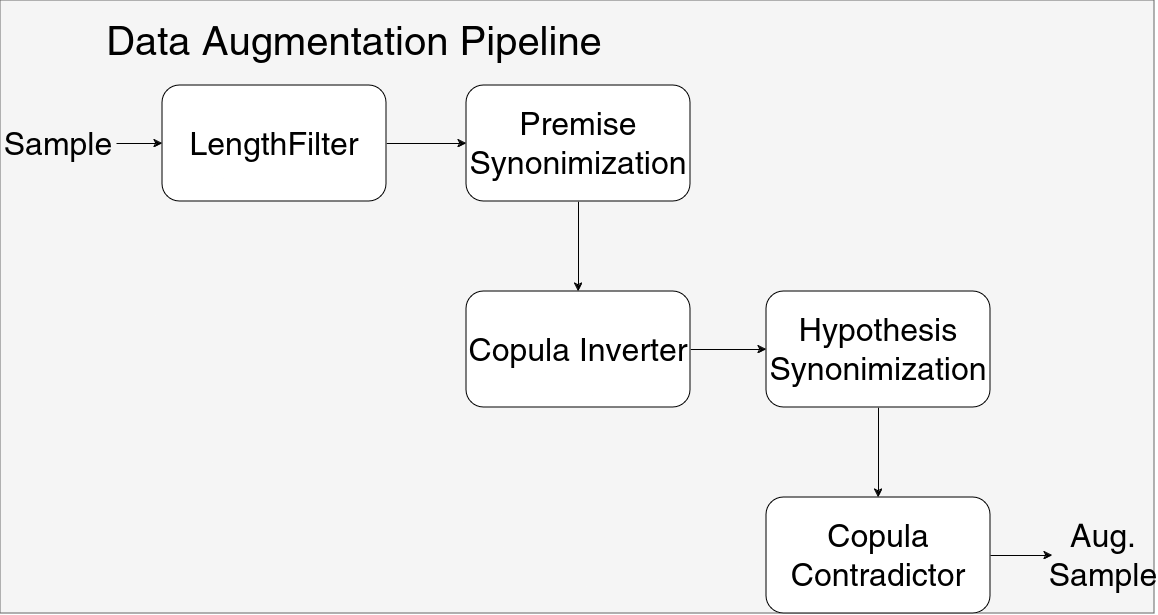
\includegraphics[width=0.8\textwidth]{images/pipeline.png}
    \caption{Augmentation pipeline.}
    \label{fig:pipeline}
  \end{figure}

\end{frame}

\begin{frame}
  \frametitle{Transformations}

  As shown in the figure, we implemented four transformations:

  \begin{enumerate}
    \item<1->


          \texttt{Synonimization}: This transform uses WSD information to produce a set of sentences where some tokens are replaced with their synonyms.
    \item<2-> \texttt{CopulaContradictor}: This transform replaces the copula in the sentence with its negation, while also negating the hypothesis (\texttt{ENTAILMENT} $\leftrightarrow$ \texttt{CONTRADICTION}).
    \item<3-> \texttt{CopulaInverter}: This transform switches the subject and the object of the copula in the sentence, preserving the entailment relation.
    \item<4-> \texttt{LengthFilter}: This transform discards samples that have different token lengths in the WSD and SRL annotations.
  \end{enumerate}



\end{frame}

\begin{frame}
  \frametitle{Models}

  We trained two models (as asked by bonus task 2):

  \begin{enumerate}
    \item A \alert{baseline} on the train set of FEVER.
    \item An \alert{augmented} model on a concatenation of the train and augmented sets.
  \end{enumerate}

  Both were fine-tunings of the \texttt{distillRoBERTa-base} model. We chose RoBERTa as
  the focus of the task is on the production of a robust model, we opted for a distilled
  version due to our limited resources.

\end{frame}

\begin{frame}
  \frametitle{Test Sets}

  The final metrics are reported on \alert{two} test sets, the first is the default
  FEVER test set, and the second is the \alert{adversarial} test set that was provided
  to us. We assume that the augmented model will be more \alert{robust} to the adversarial
  test set.

\end{frame}

\begin{frame}
  \frametitle{Results}

  We report our results in \cref{tab:results_base,tab:results_adv}.

  \begin{table}[h]
    \centering
    \caption{Results on the base test set} \label{tab:results_base}
    \begin{tabularx}{0.90\linewidth}{|X|c|c|c|c|}
      \hline
      \textbf{Model} & \textbf{Accuracy} & \textbf{Precision} & \textbf{Recall} & \textbf{F1} \\
      \hline
      \hline
      Baseline       & 0.704             & 0.699              & 0.704           & 0.694       \\
      Augmented      & 0.683             & 0.681              & 0.683           & 0.672       \\
      \hline
    \end{tabularx}
  \end{table}

  \begin{table}[h]
    \centering
    \caption{Results on the adversarial test set} \label{tab:results_adv}
    \begin{tabularx}{0.90\linewidth}{|X|c|c|c|c|}
      \hline
      \textbf{Model} & \textbf{Accuracy} & \textbf{Precision} & \textbf{Recall} & \textbf{F1} \\
      \hline
      \hline
      Baseline       & 0.496             & 0.511              & 0.496           & 0.495       \\
      Augmented      & 0.519             & 0.542              & 0.519           & 0.522       \\
      \hline
    \end{tabularx}
  \end{table}
\end{frame}


\begin{frame}
  \frametitle{Conclusions}

  It appears that our augmentation strategies \alert{improved} the robustness of the model
  to adversarial data, however, we lost a bit of performance on the base test set. As our
  task is to improve the model's generality, we consider this a \alert{success}.

\end{frame}

\begin{frame}
  \frametitle{The End!}

  \centering
  \Huge{\alert{Thank you for your attention!}}

\end{frame}

\end{document}
